\chapter{负例采样算法研究}
\label{cha:thirdsection}
本章聚焦推荐系统中的伪负例问题。隐式反馈数据面临的一个突出问题是负例未标注。通常,未交互的物品被当作负样本以训练模型。然而,其中存在没曝光给用户,但是用户可能喜欢的物品,从而导致了伪负例问题。这一问题在自监督学习的诸多领域具有普遍性,例如在自然语言处理(NLP)中,正样本可以从上下文中获得,而负样本则是从未标注的词库中随机抽样得到的。在计算机视觉(CV)中,正样本通过数据增强获得,而负样本则从未标记的图像中抽样得到。这样的数据集也被称为Positive-Unlabeled (PU)数据集。如何从未标记的数据中采样高质量的负实例,即负采样,对于训练基于对比学习的模型非常重要。本章聚焦于推荐系统中负采样问题的研究,通过设计最优负采样准则,采样信息量大且用户不喜欢的硬负样本(hard negative),以提升推荐精度。
\begin{figure*}[h!]
	\centering
	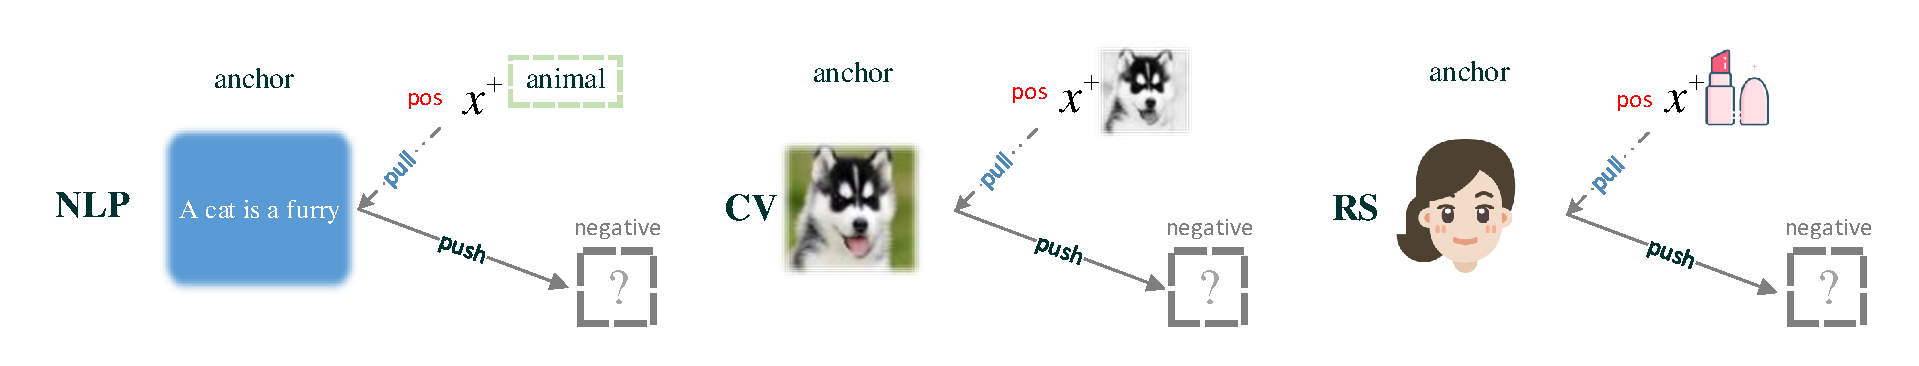
\includegraphics[width=\textwidth]{3-PU.pdf}
	\caption{Positive-Unlabeled(PU)问题示意图}
	\label{Fig:falsen}
\end{figure*}
\section{引言}
负采样源自Positive-Unlabeled (PU)问题~\cite{Jessa:2020:ML,Su:2021:IJCAI}。一个典型的PU数据集,通常只有部分正例被标注,其余样本未标注,而这些未标注的样本可能属于正类或负类。负采样,即确定从PU数据集中采样负例的策略,以便有效地训练下游任务模型。负采样在许多任务中都有广泛应用,例如自然语言处理(NLP)\cite{Mikolov:2013:NIPS,Tang:2015:WWW},计算机视觉(CV)\cite{Qin:2021:AAAI,Zhao:2021:IJCAI},以及推荐系统(RS)~\cite{Steffen:2014:WSDM,Zhang:2013:SIGIR,Ding:2020:NIPS}。本章聚焦于推荐系统中的负采样。对于一个特定的用户,他未交互的物品,称为他的\textit{负例}。里面包含用户确实不喜欢的物品,称为\textbf{真负例};也包含用户喜欢的物品,称之为\textbf{伪负例}(即正例)。负采样的困境在于,未标注的样本中含有用户潜在喜欢的伪负例,一旦这类用户感兴趣的样本被采样当作负例用于训练模型,会使得模型误判用户的兴趣边界。这激发了负采样用于推荐的问题,即如何有效地采样负实例来训练推荐模型。许多研究表明,负采样对于提高推荐性能非常重要~\cite{Steffen:2014:WSDM,Zhang:2013:SIGIR,Ding:2020:NIPS,Park:2019:WWW,Huang:2021:KDD,Ding:2019:IJCAI,Yang:2020:KDD}。

负采样算法在推荐系统中被广泛研究。根据抽样分布是否随模型状态的变化,可以将现有的负采样算法分为以下两类:\textit{静态负采样}\cite{Steffen:2009:UAI,Chen:2017:KDD,Mikolov:2013:NIPS,Xiangnan:2020:SIGIR,Weike:2013:IJCAI,Yu:2018:CIKM,Wang:2019:SIGIR}。这类算法根据固定的采样分布,如均匀采样,依物品流行度的采样等,这类抽样分布所参照的信息是静态的,不随模型训练的参数变化而变化。另外一类是\textit{动态负采样}\cite{Steffen:2014:WSDM,Zhang:2013:SIGIR,Wang:2020:WWW,Chen:2019:WWW}。这类负采样算法的抽样分布会根据模型训练不断调整,偏好于采样在嵌入空间中与正例表示更相似的负例,即难以区分的困难样本(hard negative sample),例如采样分数更高或排名更高的实例~\cite{Steffen:2014:WSDM,Zhang:2013:SIGIR,Zhao:2015:CIKM}。静态负采样可以使用某些辅助信息,免于采样到用户感兴趣的伪负例。但是由于其抽样分布是静态的,往往只会采样容易样本,不利于模型性能的提升;动态负采样可以根据模型的训练针对困难样本进行采样,更容易受到负采样问题的困扰~\cite{Ding:2020:NIPS,Qin:2021:AAAI,Zhao:2021:IJCAI}。

本章对推荐系统的负采样研究做出了以下三个方面的贡献:(1) 根据经验分布函数的渐近性质,定义了一个与模型无关的负信号测度,用于度量未标注样本是真负例的后验概率。特别地,它较好地结合了现有基于先验信息(与模型无关)以及基于样本信息(与模型相关)的两种提取负信号的范式。 (2) 本章还提出了最优采样准则,用于采样高质量的负例。这是一个经验采样风险最小化的理论最优采样准则。实验证明了所提出的负采样算法在采样质量和推荐性能方面的有效性。

\section{负采样分析}
对于一个由$M$个用户和$N$个物品组成用户-物品交互矩阵$\mathbf{X}=[x_{ui}] \in \mathbb{R}^{M\times N}$,元素$x_{ui}=1$表示用户$u$与物品$i$有交互;否则,$x_{ui}=0$。为了训练推荐模型 $\mathcal{M}$,我们考虑如下广泛使用的BPR优化目标:
\begin{equation}\label{Eq:PairewiseLossFunction}\
	\mathcal{L} = \sum_{(u,i,j)} \ln \sigma(\hat{x}_{ui} - \hat{x}_{uj}) ,
\end{equation}
对于用户 $u$,其中 $\hat{x}_{ui}$ 和 $\hat{x}_{uj}$ 分别是他已交互物品 $i$ 和未交互物品 $j$ 的预测分数,由用户物品表示$\Theta$参数化:$\hat{x}_{ui} = \mathtt{sim}(\mathbf{w}_u, \mathbf{h}_i)$,其中 $\mathtt{sim}$ 是相似度函数,例如余弦相似度或点积函数。$(u,i,j)$为训练三元组。训练三元组 $(u,i,j)$ 的构建如下:对于用户 $u$ 和他的一个正例 $i \in \mathcal{I}_u^+$,负例从未标注样本中随机采样一个 $j \in \mathcal{I}_u^-$,即进行负采样。存在着两种情况,即用户 $u$ 实际上喜欢$j$,未交互仅仅是因为之前没有看到过它,也就是说,物品 $j$ 对于用户 $u$ 来说是一个伪负例。另一方面,如果用户 $u$ 确实不喜欢物品 $j$,则该物品被称为真负例。

\par
通常使用\textit{随机梯度下降}(SGD)来迭代优化每个训练三元组 $(u, i, j)$ 的损失函数。对于采样的实例 $j \in \mathcal{I}_u^-$,如果它是用户 $u$ 的真负例,则相对于其预测得分 $\hat{x}_{uj}$ 的损失梯度计算如下
\begin{equation}\label{Eq:GradientOriginal}
	\frac{\partial \mathcal{L} }{\partial \hat{x}_{uj}} = [1-\sigma(\hat{x}_{ui} - \hat{x}_{uj})] (-1),
\end{equation}
其中 $\sigma(\cdot)$ 是 \textsf{sigmoid} 函数。然而,如果采样的实例 $j$ 实际上是一个伪负例,根据微分的链式法则,正确的梯度更新应该是相反,即公式~\eqref{Eq:GradientOriginal}的最后一项 $(-1)$改为$(+1)$。由此可见,对于一个未标注样本,由于其标签不同,梯度方向也截然相反。因此可以把损失函数相对于未标注样本地损失梯度写为:
\begin{equation}\label{Eq:Gradient}
	\frac{\partial \mathcal{L}_{loss} }{\partial \hat{x}_{uj}} = [1-\sigma(\hat{x}_{ui} - \hat{x}_{uj})] \cdot \mathtt{sgn}(j),
\end{equation}
其中,如果 $j$ 是用户 $u$ 的真负例,则 $\mathtt{sgn}(j)=-1$;如果 $j$ 是用户 $u$ 的误判负例,则 $\mathtt{sgn}(j)=1$。损失函数的梯度公式~\eqref{Eq:Gradient} 可以分解为两部分,即\textit{梯度幅度}和\textit{梯度方向}。这激发了我们对负采样的分析,即什么是高质量的负例:如果在训练三元组 $(u,i,j)$ 中采样的实例 $j$ 同时具有信息量和无偏性,那么它被称为\textit{高质量负例}。
\begin{itemize}
	\item \textbf{信息量}: 未标注样本$j$的信息量定义为该样本对应的损失函数梯度幅度的大小,即
	\begin{equation}\label{Eq:Informativeness}
		\mathtt{info}(j) =  [1-\sigma(\hat{x}_{ui} - \hat{x}_{uj})].
	\end{equation}
	\item \textbf{无偏性}: 未标注样本$j$的信息量定义为该样本是真负例的后验概率大小,即
	\begin{equation}\label{Eq:Unbiasedness}
		\mathtt{unbias}(j) = \mathrm{P}(\mathtt{sgn}(j) = -1).
	\end{equation}
\end{itemize}

信息量与未标注样本$j$ 对于推荐模型参数更新的帮助程度相关。给定正例的预测得分 $\hat{x}_{ui}$,如果未标注样本$\hat{x}_{uj}$ 的值过小,则 $\sigma(\hat{x}_{ui} - \hat{x}_{uj}) \rightarrow 1$ 且 $\mathtt{info}(j) \rightarrow 0$,即梯度消失,无法从未标注样本$j$上学到太多信息。这是困难负采样(hard negative sampling)的一个重要动机。

无偏性实际上定义为未标注样本$j$ 是真负例的概率。对于负采样而言,正例已经给定,目标是采样真负例。在训练时,把采样到的未标注样本当作负例,即直接设置 $\mathtt{sgn}(j)=-1$。当存在采样偏差时,即采样到正例,将导致推荐模型误判用户的兴趣边界。如何从未标记的样本中识别出真负例示例是必须解决的负采样关键研究问题。

采样偏差的不良影响不仅限于BPR损失,上述分析可以同样推广到其他一些基于对比的损失函数如InfoNCE,也可能因错误的负采样而受到影响:当采样一个伪负例时,损失函数对于该采样的样本梯度方向错误。这个伪负例的特征表示将被推离锚点$u$,而实际上它应该在嵌入空间中靠近锚点。

\section{贝叶斯最优负采样算法}
\subsection{类条件概率密度} \label{Sec:Dis}
由于所有未标注样本的预测得分都是使用相同的编码器和相同的得分函数预测的,因此可以假设预测得分 $\hat{x}$ 是独立同分布的,其概率密度函数记为抽象函数$f(\hat{x})$,相应的累积分布函数为 $F(\hat{x}) =\int_{- \infty }^{\hat{x}} f(t)dt$。

考虑未标注样本中的两个总体:真负例和伪负例。根据成对学习的优化目标,是针对锚点和正例的相似度分数高于负例的相似度分数进行优化。这表明以下预测得分的次序关系可能在一般情况下成立
\begin{equation}\label{Eq:OrderRelation}
	X_{tn} \leq X_{fn},
\end{equation}
其中,$X_{tn}$ 和 $X_{fn}$ 分别为真负例和伪负例(即未来测试数据中的正例)的预测得分的随机变量。需要注意的是,这也是对比学习方法~\cite{gutmann:2012:JMLR,Oord:2018:arxiv,Gutmann:2010:ICAIS} 的优化目标,其本质上鼓励学到的正例特征表示与“锚点”数据点相似,同时将负例特征与“锚点”数据在嵌入空间中推远,使其不相似\cite{Wang:2020:ICML,Xu:2022:arxiv,Liu:2021:TKDE}。

真负例和伪负例两个总体预测分数的这种序关系,可以使用次序统计量的技术写出真负例和伪负例这两个总体相似度分数分布:
\begin{eqnarray}\label{Eq:TNpdf}
g(\hat{x}_{tn}) &=& 2 f(\hat{x}_{tn}) [1 - F(\hat{x}_{tn})],\\
h(\hat{x}_{fn}) &=& 2 F(\hat{x}_{fn}) f(\hat{x}_{fn}).	
\end{eqnarray}
\subsubsection{经验分布}\label{Appendix:Realdist}
为了验证公式~\eqref{Eq:OrderRelation} 的次序关系,在模型训练过程中记录真负例总体(TN)和伪负例总体(FN)相似度分数的经验分布。其中,伪负例总体是测试集中的物品,在训练过程中无法观测;真负例总体是未交互物品中,除去测试集之外的其余物品。在MovieLens-100K数据集上,采用经典的矩阵分解推荐模型,并采用随机负采样在训练集上训练模型,并记录每个训练周期的预测得分。通过统计真负例和误判负例的预测得分,在图~\ref{Fig:DistributionStatistics} 中报告了它们在模型训练中的分布密度。
\begin{figure*}[h!]
	\centering
	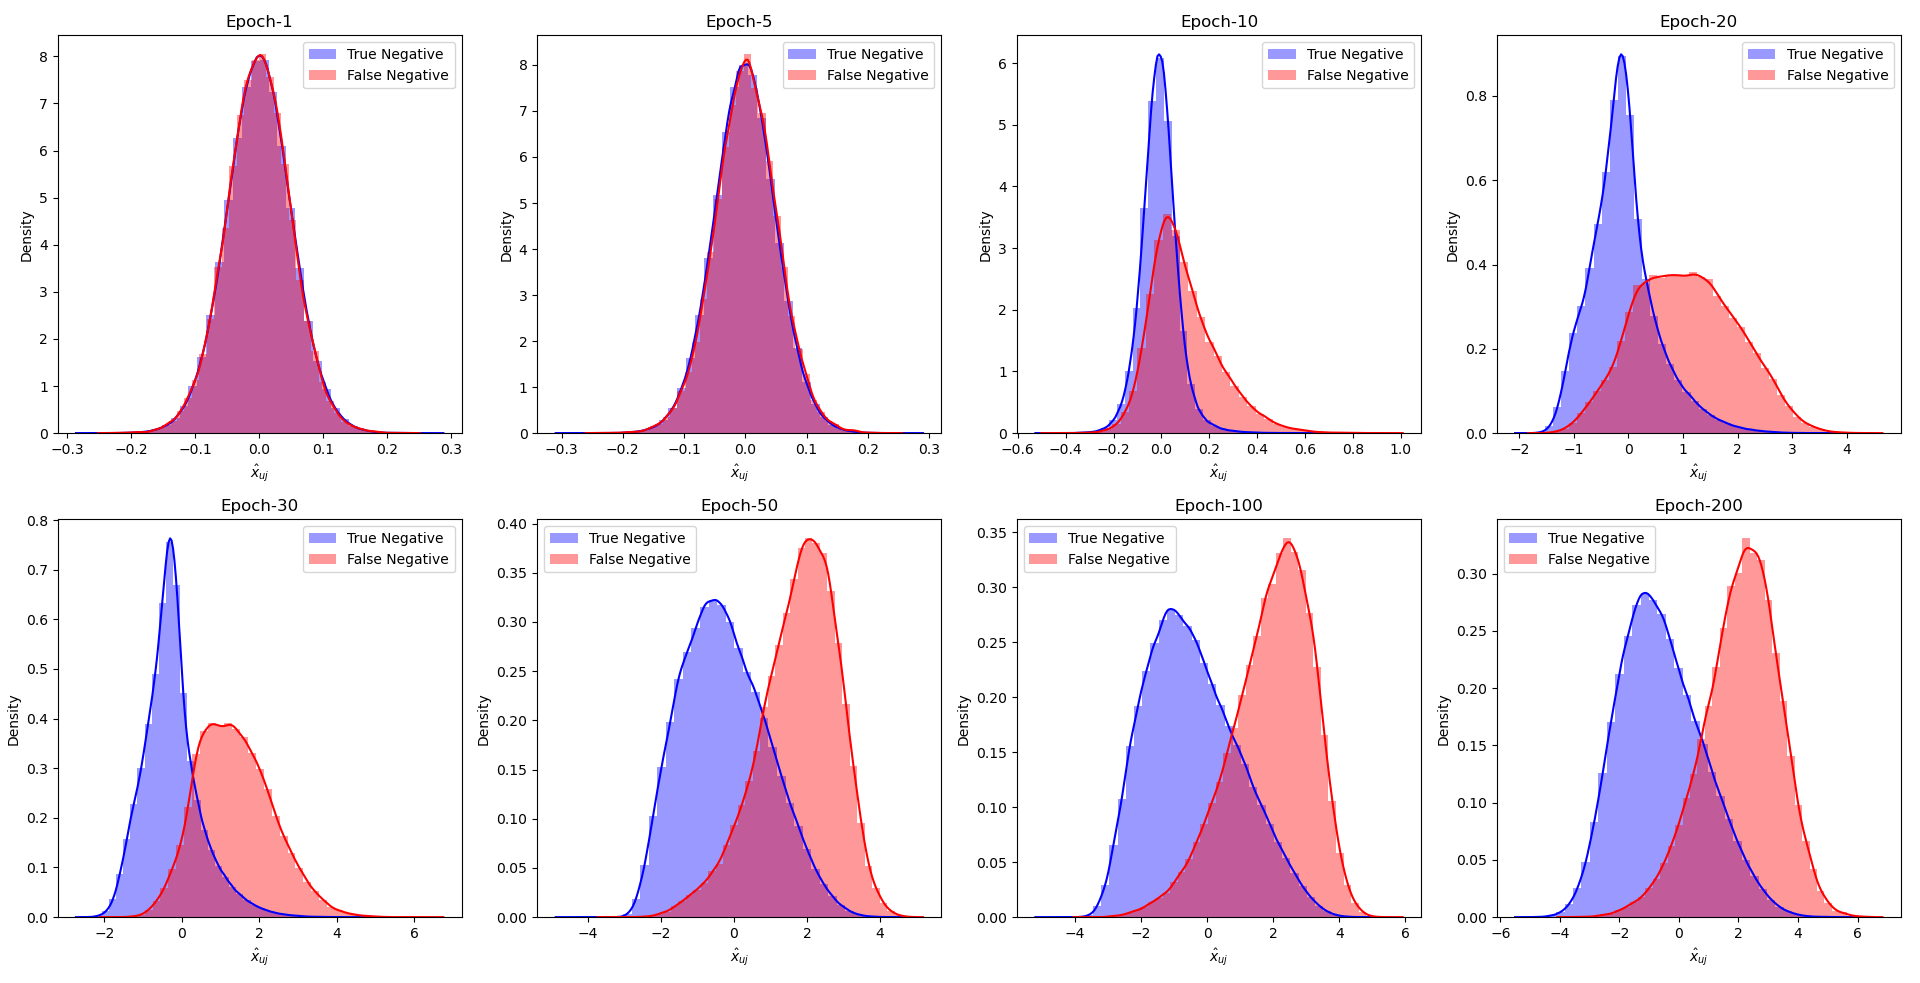
\includegraphics[width=\textwidth, height=0.5\textwidth]{3-DistributionStatistics1.png}
	\caption{不同训练时点的相似度分数的经验分布}
	\label{Fig:DistributionStatistics}
\end{figure*}
\par
图~\ref{Fig:DistributionStatistics} 提供了两个发现:
\begin{itemize}
\item 负例的预测得分越高,它是伪负例的概率密度就越高,而是真负例的概率密度就越低;
\item 随着训练的进行,两个分布之间的区别逐渐变得更加清晰:与真负例相比,伪负例的分布集中在更高的得分上。这表明,相对于真负例而言,推荐模型总体上能够给伪负例更高的评分。
\end{itemize}

\subsubsection{理论分布}\label{Appendix:Theodist}
\begin{figure}[h!]
	\centering
	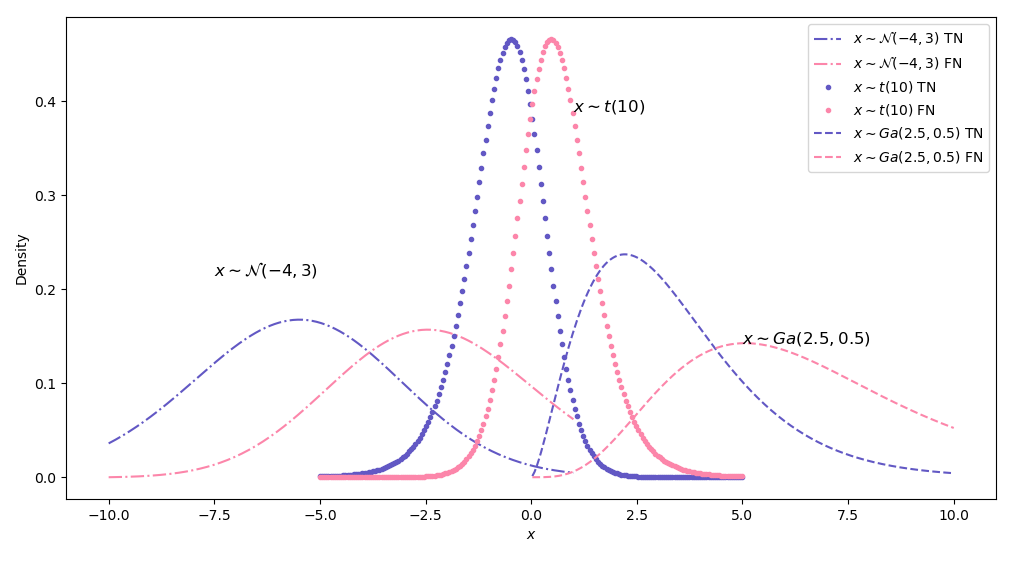
\includegraphics[width=.9\textwidth, height=0.45\textwidth]{3-theorydist.png}
	\caption{相似度分数的理论分布}
	\label{Fig:TheoryDist}
\end{figure}
图~\ref{Fig:TheoryDist} 展示了基于不同类型的分布$f(x)$时(高斯分布 $x\sim \mathcal{N}(\mu,\sigma)$,学生分布 $x\sim t(n)$ 和伽玛分布 $x\sim Ga(\alpha,\lambda)$),公式\eqref{Eq:TNpdf}所对应的真负例和伪负例的分数分布形态。在训练过程中,使用真实数据集绘制的经验分布图~\ref{Fig:DistributionStatistics},逐渐展示出了与图~\ref{Fig:TheoryDist} 中描述的理论分布出现了相同结构。

目前为止,我们还不知道 $f(x)$ 和 $F(x)$ 的显式表达式。不同的得分函数和推荐模型会产生不同的未标注样本分数密度表达 $f(\cdot)$,但这种分离的结构足以让我们对真负例和伪负例进行分类。此外,经验分布函数 $\hat F(x)= \frac{1}{n}\sum_j I_{|X_\cdot \leq \hat{x}_l|}$ 的计算很容易实现。 根据Glivenko定理~\cite{glivenko:1933},经验分布函数一致收敛于分布函数,使得可以通过计算经验分布函数,以实现对抽象函数$F(\cdot)$的近似。这一有力工具,使得本章所提出的负采样方法不再局限于简单的矩阵分解模型,可以向任何深度神经网络模型推广。

\subsection{贝叶斯分类}
对于一个未交互的物品$l$以及其对应的预测得分为$\hat{x}_l$,使用贝叶斯公式计算物品$l$为真负例的后验概率:
\begin{eqnarray} \label{Eq:PostTN}
	P(tn|\hat{x}_l) &\propto& P(\hat{x}_l|tn) P_{tn}(l) \nonumber \\
	&=&  2f(\hat{x}_l) [1 - F(\hat{x}_l)] P_{tn}(l),
\end{eqnarray}
其中,$P(\hat{x}l|tn)$ 是真负例的类条件密度,由 $g(\hat{x})$ 给出;$P_{tn}(l) = 1 - P_{fn}(l)$ 是物品 $l$ 为真负例的先验概率。$f(\hat{x}_l)$ 是所有未标注样本的得分分布,$F(\hat{x}_l) = \int_{-\infty}^{\hat{x}_l} f(t) dt$ 是相应的累积分布函数。同样地,未标注样本$l$是伪负例的后验概率为
\begin{eqnarray}\label{Eq:PostFN}
	P(fn|\hat{x}_l) &\propto& P(\hat{x}_l|fn) P_{fn}(l) \nonumber \\
	&=& 2 F(\hat{x}_l) f(\hat{x}_l) P_{fn}(l)
\end{eqnarray}

贝叶斯分类器可以通过最大化后验概率来得到:
\begin{eqnarray}
	\mathop{\arg\max}\limits_{c \in \{fn, tn\}} P(c|\hat{x}_l).
\end{eqnarray}

直接计算公式~\eqref{Eq:PostTN} 和公式~\eqref{Eq:PostFN} 中的得分密度函数 $f(\cdot)$ 并不实际。然而,计算经验分布函数却很容易实现。因此,使用贝叶斯公式的分式形式定义无偏性,以消除密度函数 $f(\cdot)$:
\begin{eqnarray}
	\mathtt{unbias}(l) &\triangleq&  P(tn|\hat{x}_l) = \frac{P(tn,\hat{x}_l)}{P(\hat{x}_l)} \label{Eq:NorPost} \\
	&=& \frac{P(\hat{x}_l |tn)P_{tn}(l)}{P(\hat{x}_l |tn)P_{tn}(l)+P(\hat{x}_l |fn)P_{fn}(l)} \\
	&=& \frac{ f(\hat{x}_l) [1 - F(\hat{x}_l)] P_{tn}(l)}{ f(\hat{x}_l) [1 - F(\hat{x}_l)] P_{tn}(l) + F(\hat{x}_l) f(\hat{x}_l) P_{fn}(l) }  \nonumber\\
	&=&  \frac{  [1 - F(\hat{x}_l)][1-P_{fn}(l)] }{1 - F(\hat{x}_l) -P_{fn}(l) + 2F(\hat{x}_l)P_{fn}(l) }.\label{Eq:unbias}
\end{eqnarray}
根据 Glivenko 定理~\cite{glivenko:1933},可以使用 $\hat F(\hat{x}_l)$ 来近似 $F(\hat{x})$,即 $\hat{x}_{\cdot} \leq \hat{x}_l$的比例:
\begin{eqnarray}\label{Eq:CDF}
 F(x) \simeq \frac{1}{n}\sum_j I_{|X_\cdot \leq \hat{x}_l|}
\end{eqnarray}
$P_{fn}(l)$ 是物品 $l$ 为伪负例的先验概率。假设物品 $l$ 被交互的次数 $pop_l \sim B(N, P_{fn}(l))$,其中 $N$ 是训练集中的总交互次数。那么,
\begin{eqnarray}\label{Eq:Prior}	
	P_{fn}(l) = \frac{pop_l}{N}.
\end{eqnarray}

%\begin{lemma}[Unbiased negative signal]\label{unbias}
%	If $pop_l \sim B (N, P_{fn}(l))$, then $\mathtt{unbias}(l)$ measure given by Eq~\eqref{Eq:unbias} is an unbiased estimator for $l$ being true negative.
%	
%	\begin{proof}
%		Setting random variable $Y=1$ if $l \in fn$, otherwise $Y=0$,
%		\begin{eqnarray}
%			Y= \left\{
%			\begin{aligned}
%				1 ,~ P &=& \theta \\
%				0 ,~ P &=& 1-\theta, \\
%			\end{aligned}
%			\right.
%		\end{eqnarray}
%		where $\theta$ is the probability of $l$ being false negative. So $Y \sim B(1,\theta)$. $pop_l = Y_1 + Y_2 + \cdots + Y_N  \sim B(N,\theta)$, then $P(pop_l=k )= \binom{N}{k} \theta^k (1-\theta)^{(N-k)} $. So
%		
%		\begin{eqnarray}
%			\mathbb{E}[P_{fn}(l)] &=& \mathbb{E}(\frac{pop_l}{N}) \nonumber \\
%			&=& \theta
%		\end{eqnarray}
%		
%		Given the observation $ X = \hat{x}_{ul}$, $F(X)$ is a statistic of $X$. $P_{fn}(l)$ is a statistic of $\sum_i Y_i$ that is independent of $X$. So
%		\begin{eqnarray}
%			&&\mathbb{E} [\mathtt{unbias}(l)]  \nonumber \\
%			&=& \mathbb{E}   \frac{  [1 - F(X)][1-P_{fn}(l)] }{1 - F(X) -P_{fn}(l) + 2F(X)P_{fn}(l) } \nonumber  \\
%			&=&  \frac{  [1 - \mathbb{E}  [F(X)]] [1- \mathbb{E} [ P_{fn}(l)]] }{1 -\mathbb{E} [F(X)] - \mathbb{E}[P_{fn}(l)] + \mathbb{E} [2F(X)P_{fn}(l)] }
%		\end{eqnarray}
%		$\mathbb{E}[F(X)]$ is the first order origin moment of cumulative distribution function $F(X)$
%		\begin{eqnarray}
%			\mathbb{E}  [F(X)] &=& \int_{-\infty}^{\infty} F(x) f(x) dx\nonumber\\
%			&= &  \int_{-\infty}^{\infty} F(x) dF(x)\nonumber\\
%			&= &  \frac{1}{2}  F^2(x)   \bigg|_{x=-\infty}  ^{x=\infty} \nonumber\\
%			&= & \frac{1}{2}.
%		\end{eqnarray}
%		So
%		\begin{eqnarray}
%			\mathbb{E} [\mathtt{unbias}(l)] &=&  \frac{  (1 - \frac{1}{2}) (1-\theta) }{1 -\frac{1}{2} - \theta + 2\cdot \frac{1}{2} \cdot \theta} \nonumber  \\
%			&=& 1-\theta.
%		\end{eqnarray}
%		Note $1-\theta$ is the probability of $Y=0$ from binomial populations $Y\sim B(1,\theta)$, so $\mathtt{unbias}(l)$ is unbiased estimator of $l$ being true negative. Fig~\ref{Fig:unbias} plots $\mathtt{unbias}(l)$ as a function of $F(\hat{x}) \in [0,1]$ and $P_{fn}(l) \in [0,1]$. We observe that $\mathtt{unbias}(l)$ is a decreasing function w.r.t both $F(\hat{x})$ and $P(fn)$. The monotonicity of $\mathtt{unbias}(j)$ is consistent with our analysis, and the value domain of $\mathtt{unbias}(j)$ $\in [0,1]$ conforms to the probability form.
%		\begin{figure}[h]
%			\centering
%			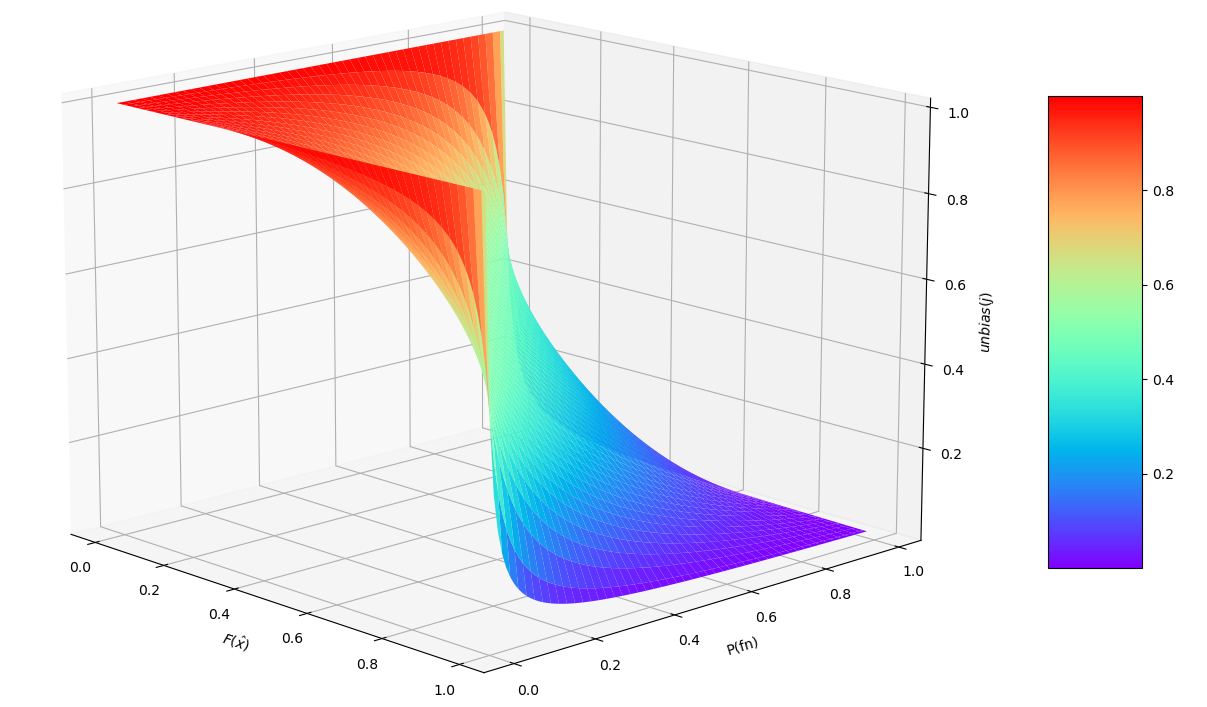
\includegraphics[width=0.4\textwidth]{3-unbias.png}
%			\caption{Numerical plots of posterior probability $\mathtt{unbias}(j)$ by Eq.~\eqref{Eq:unbias}.}
%			\label{Fig:unbias}
%		\end{figure}
%	\end{proof}
%\end{lemma}

无偏性的定义是物品$l$ 为真负例的后验概率。由于公式~\eqref{Eq:unbias}的分数表达式,未标注样本分数的密度函数 $f(\hat{x}_l)$ 被消除掉。公式~\eqref{Eq:unbias} 意味着未交互物品 $l$ 的负信号形式上由以下因素决定:(i) 推荐模型输出的排序位置,用 $F(\hat{x}_l)$ 表示,其中排序位置和 $F(\hat{x}_l)$ 具有一一映射关系。较大的 $F(\hat{x}_l)$,即靠前的的排序位置,表明推荐模型在很大程度上将 $l$ 分类为用户感兴趣的伪负例(正例),即$F(\hat{x}_l)$ 分配了一个在 $[0,1]$ 范围内的$l$ 是伪负例(正例)的概率预测。这解释了为什么那些过采样得分较高或排名较高的困难负例的算法~\cite{Steffen:2014:WSDM,Zhang:2013:SIGIR} 更容易采样伪负例的问题。(ii)先验信息,表示为先验概率($P_{tn}(l)$ 或 $P_{fn}(l)$)。

注意到,公式~\eqref{Eq:unbias} 的度量标准统一了当前关于提取负信号的两种主要范式:(i)建模先验信息,如 曝光数据~\cite{Jingtao:2019:IJCAI}、知识图谱实体~\cite{Wang:2020:WWW}、社交网络中的连接~\cite{Zhao:2014:CIKM,Wang:2016:CIKM} 等;(ii) 建依赖模型的样本信息,如预测得分~\cite{Steffen:2014:WSDM}、排名位置~\cite{Zhang:2013:SIGIR}、得分方差~\cite{Ding:2020:NIPS} 等。前者可以融入领域知识,但负信号与模型状态无关;后者利用样本信息 $\hat{x}_l$,但忽略了先验信息。$\mathtt{unbias}(\cdot)$ 测度的优势在于其对应的后验概率的理论解释:它结合了先验信息(与模型无关)和样本信息 $\hat{x}_l$(与模型相关)。本章只是为了简化,采用了一种简单的方法来建模先验概率,但不局限于此,$P_{tn}(l)$为使用其他附加信息和领域知识来建模先验概率提供了灵活的接口。

\subsection{最优采样准则}
公式~\eqref{Eq:PairewiseLossFunction}的成对损失$\mathcal{L}$ 可以类比于$AUC$ 指标~\cite{Steffen:2009:UAI}。它用可微的损失函数 $\ln \sigma(\cdot)$ 替代了 $AUC$ 指标中的不可微的0-1损失,这在优化 $AUC$ 时是一种常见做法~\cite{Herschtal:2004:ICML,Steffen:2009:UAI},因此关心$\mathcal{L}$的大小也是关心AUC指标的大小。

先在给定正例对$(u,i)$,采样到的样本$l$ 直接被赋予一个负向的梯度,导致预测得分 $\hat{x}_{ul}$ 的减少,这会对 $\mathcal{L}$ 产生两种影响:(i)当$l$是伪负例时,$\mathcal{L}$会减少,表示为 $\triangle \mathcal{L}_{fn}(l|i)$;(ii) 当$l$是真负例时,$\mathcal{L}$会增加,表示为 $\triangle \mathcal{L}_{tn}(l|i)$。

\begin{definition}[条件采样风险]
对于给定的正例对$(u,i)$,定义采样未标注样本$l$ 的条件采样风险为,采样损失$\triangle \mathcal{L}(l|i)$相对于$l$的标签$c$的期望值:
	\begin{eqnarray}
		R(l|i) 
		&=&  \mathbb{E}_{l \sim P(c|l)}  \triangle \mathcal{L}(l|i)\nonumber\\
		&=&[1- P(tn|l)] \cdot \triangle \mathcal{L}_{fn}(l|i) + P(tn|l)\cdot \triangle \mathcal{L}_{tn}(l|i)\label{eq:condirisk},
	\end{eqnarray}
其中$P(tn|l)$是$l\in tn$的后验概率,可以使用$\mathtt{unbias}(l)$计算, $ 1 - P(tn|l)$是$l\in fn$的后验概率。条件采样风险的的含义是,给定正例$i$,采样$l$所带来的AUC的期望减小值。
\end{definition}

\begin{definition}[经验采样风险]
采样器 $h$ 的经验采样风险为,条件采样风险$R(l|i)$对所有正例分布的期望值:
	\begin{eqnarray}
		R(h) = \mathbb{E}_{i \sim P(i)} R(l|i).
	\end{eqnarray}
经验采样风险的含义为,对于所有正例,采样器所带来的AUC的期望减小值。
\end{definition}
任务是找到一个采样策略 $h:\mathcal{I}_u^- \rightarrow l$,以最小化经验采样风险,从而实现最大化AUC。如下定理给出了经验采样风险最小化意义的最优采样准则:
\begin{theorem}[最优采样准则] \label{optimalrule}
若条件采样风险$R(l|i)$相互独立, 那么对任意采样器$h: \mathcal{I}_u^- \rightarrow l$,
	\begin{eqnarray}\label{Eq:OptimalSam}
		h^* &=&   \mathop{\arg\min}\limits_{l \in\mathcal{I}_u^-} R(l|i)
	\end{eqnarray}
是最小化经验采样风险的最优采样策略。
	\begin{proof}
给定训练集,正样本的分布 $P(i)$ 是确定的。那么经验采样风险是
		\begin{eqnarray}
			R(h) = \mathbb{E}_{i \sim P(i) } R(h|i)
		\end{eqnarray}
其中$R(h|i)$是给定正例$i$的条件采样风险。于是
		\begin{eqnarray}
	R(h^*) - R(h)
			&=&	\mathbb{E}_{i \sim P(i) }  R(h^*|i) - \mathbb{E}_{i \sim P(i) }  R(h|i)  \nonumber \\
			&=& \sum_i P(i)  [R(h^*|i) - R(h|i)] \nonumber \\
			&=& \sum_i P(i)  [  \mathop{\arg\min}\limits_{l \in\mathcal{I}_u^-} R(l|i)  - R(h|i)]\nonumber \\
			&\leq& 0.
		\end{eqnarray}
因此,经验采样风险的下确界可以表示为最优采样器 $h^*$ 的形式:
		\begin{eqnarray}
			\inf \{R(h)\} 	&=& R(h^*) \nonumber\\
			&=& \mathbb{E}_{i \sim P(i) } R(h^*|i).
		\end{eqnarray}
	\end{proof}
证毕。
\end{theorem}
这个结论是直观的:如果采样器 $h^*$ 最小化了条件采样风险 $R(l|i)$,那么经验采样风险也将被最小化。

接下来将估计采样负例实例 $l$ 的采样损失 $\triangle \mathcal{L}(l|i)$。为了简化分析,我们遵循~\cite{Steffen:2009:UAI} 的独立性假设,只考虑单个成对比较损失$\tilde{\mathcal{L}}= \ln \sigma(\hat{x}_{fn} - \hat{x}_{tn})$ 的变化值。$\tilde{\mathcal{L}}$ 关于点 $\hat{x}_{ul}$ 的泰勒展开式为:





\begin{eqnarray}
	\tilde{	\mathcal{L}}' =\left\{
	\begin{aligned}
		\tilde{\mathcal{L}} +  \frac{\partial \mathcal{L}} {\partial \hat{x}_{ul}}  ( \hat{x}_{ul}' - \hat{x}_{ul}) + o( \hat{x}_{ul}' - \hat{x}_{ul}) ,~ &if&~ l \in fn\\
		\tilde{\mathcal{L}} -  \frac{\partial \mathcal{L}} {\partial \hat{x}_{ul}}  ( \hat{x}_{ul}' - \hat{x}_{ul}) + o( \hat{x}_{ul}' - \hat{x}_{ul}) ,~ &if&~ l \in tn.\\
	\end{aligned}
	\right.
\end{eqnarray}
其中 $ \frac{\partial \mathcal{L}} {\partial \hat{x}_{ul}} =  \mathtt{info}(l) $。因此单位减量$\hat{x}_{ul}$ (i.e., $\triangle \hat{x}_{ul}=-1$) 导致 $\triangle \mathcal{L}_{fn}(l|i) = \tilde{\mathcal{L}}-\tilde{\mathcal{L}}' \approx \mathtt{info}(l)$, 含义为$\tilde{\mathcal{L}}$ 减少,若$l$是伪负例; 否则$\mathcal{L}_{tn}(l|i)  \approx -\mathtt{info}(l) $,含义为$\tilde{\mathcal{L}}$的增加。为了把所有有序对的$\mathcal{L}$值纳入考虑,我们引入一个超参数 $\lambda$ 来控制效果的相对大小,并估计采样损失为:
\begin{eqnarray} \label{Eq:rankinggain}
	\triangle	\mathcal{L}(l|i)  \approx \left\{
	\begin{aligned}
		\mathtt{info}(l) ,~ &if&~ l \in fn\\
		- \lambda \mathtt{info}(l) ,~ &if&~ l \in tn\\
	\end{aligned}
	\right.
\end{eqnarray}
那么,给定正例$i$,$l$的条件采样风险为:
\begin{eqnarray}
	R(l|i) = P(fn|l) \cdot \mathtt{info}(l) - P(tn|l)\cdot \lambda\mathtt{info}(l).
\end{eqnarray}

因此,负采样通过选择条件采样风险最小的样本实现:
\begin{eqnarray} \label{Eq:NegativeSam}
	j   &=&   \mathop{\arg\min}\limits_{l \in \mathcal{M}_u} R(l|i) \nonumber \\
	&=& \mathop{\arg\min}\limits_{l \in \mathcal{M}_u}~ [1-\mathtt{unbias}(l)] \cdot \mathtt{info}(l)- \lambda \cdot \mathtt{unbias}(l) \cdot \mathtt{info}(l)  \nonumber \\
	&=& \mathop{\arg\min}\limits_{l \in\mathcal{M}_u}~ \mathtt{info}(l)\cdot [1-(1+\lambda)\mathtt{unbias}(l)]
\end{eqnarray}
其中$\mathcal{M}_u \subseteq  \mathcal{I}_u^-$是一个从未交互物品集合$\mathcal{I}_u^-$中随机采样的小的候选集。当 $|\mathcal{M}_u| = |\mathcal{I}_u^-|$时, 此时采样器即为经验采样风险最小的理论最优采样器; 当$\lambda \rightarrow \infty$时, $h$ 退化为$\mathop{\arg\max}\limits_{l \in\mathcal{M}_u} \mathtt{info}(l)\cdot \mathtt{unbias}(l)$, 即采样信息量大(即困难样本)且无偏的(即用户不喜欢)的样本。由于采样准则的实现依赖于结合了先验信息和样本信息的负信号测度$\mathtt{unbias}(l)$,因此称本章提出的方法为贝叶斯负采样算法(Bayesian Negative Sampling, BNS)。

\section{算法实现与时间复杂度分析}
\subsection{算法步骤}
BNS也隶属于动态负采样算法的一种,需要根据样本的预测评分进行采样,因此抽样分布会随着模型训练而变化,因此和典型的动态负采样算法一样,BNS首先需要计算用户的评分向量。本章提出的负例采样算法实现步骤总结如下:对于候选集合 $\mathcal{M}_u$ 中的每个负例实例:(1)计算先验概率,(2)计算经验分布函数$F(\hat{x}_l)$。它反映了模型对未标注样本$l$所属类别的判别。未标注样本$l$的预测评分越高(困难负样本),表明模型认为用户喜欢这个物品,$F(\hat{x}_l)$值越接近于1,即伪负例的概率越高。(3)计算样本是真负例的后验概率 $\mathtt{unbias}(l)$。(4)根据公式~\eqref{Eq:NegativeSam} 进行负例采样。它实际上是通过选择一个未标注样本,最大化了下一个训练轮次的AUC和当前训练轮次的AUC差值。算法~\ref{Alg:1} 给出了提出的负采样算法的伪代码。


\subsection{时间复杂度}
第一步计算先验概率,由于先验概率是静态的,时间复杂度为 $\mathcal{O}(1)$。在本章中,使用流行度建模,只需要常数次操作即可实现。第二部计算经验分布函数,时间复杂度为 $\mathcal{O}(\vert\mathcal{I}\vert)$)。第三步计算后验概率,时间复杂度为 $\mathcal{O}(1)$;第四步,执行贝叶斯负采样,对于规模为$m$的候选集,需要执行$m$次操作,时间复杂度为 $\mathcal{O}(1)$。因此,提出的贝叶斯负采样算法\textsf{BNS}相对于物品个数$|\mathcal{I}|$具有线性时间复杂度。

相比于静态负采样算法,以BNS为代表的动态负采样算法有额外的计算开销,主要体现在两点:(1)计算用户的评分向量。从模型训练的角度而言,正向传播实际上只需要计算正负两个样本的预测得分,就可以反向传播更新参数。但是动态负采样由于需要采样困难负样本,所以需要计算其它额外的候选负例评分,从而产生了额外的计算开销。(2)计算经验分布函数。$m$个候选样本需要计算$m$次经验分布函数。但是需要强调的是,计算用户的评分向量时间复杂度通常远大于计算经验分布函数,前者是矩阵运算,后者是标量运算。




\begin{algorithm}[!]
	\small
	\caption{贝叶斯负采样算法(BNS)伪代码}\label{Alg:1}
	\KwIn{交互集合$\mathcal{R}=\{(u,i)\}$, 评分函数$s(\cdot)$, 候选集$\mathcal{M}_u$的大小$m$,  权重$\lambda$。}
	\KwOut{模型参数$\Theta \in \mathbb{R}^d$}
	\For{$epoch=1, 2, ..., T$}{
		~~随机采样一个mini-batch $\mathcal{R}_{batch} \in \mathcal{R}$\\
		\For{每个交互$(u,i) \in \mathcal{R}_{batch}$}{
			计算评分向量 $\hat{\mathbf{x}}_u$ . \label{Algo:rating}\\
			$\backslash$$\backslash$ $\textit{开始负采样}$ \\
			均匀采样候选集$\mathcal{M}_u \subseteq  \mathcal{I}_u^-$. \label{Algo:candi} \\
			\For {每个候选负例 $(u,l) \in \mathcal{M}_u$}{
				~~通过公式\eqref{Eq:Informativeness}计算$\mathtt{info}(l)$; \label{Algo:inf} \\
				通过公式\eqref{Eq:Prior}计算$P_{fn}(l)$; $\backslash$$\backslash$~\textit{先验} \label{Algo:p} \\
				通过公式~\eqref{Eq:CDF}计算$F(\hat{x}_l)$; $\backslash$$\backslash$~\textit{似然}\label{Algo:f} \\	
				通过公式~\eqref{Eq:unbias}计算$\mathtt{unbias}(l)$; $\backslash$$\backslash$~\textit{后验} \label{Algo:unbias} 
			}
			~~根据采样准则\eqref{Eq:NegativeSam}采样$j$;\label{Algo:samp} \\
			更新用户、物品表示$\mathbf{w}_u, \mathbf{h}_i, \mathbf{h}_j$.}
	}
	\KwResult{用户和物品特征表示$\Theta$。}
\end{algorithm}
\section{试验评估}
\subsection{试验设置}
\subsubsection{数据集}
本章在三个公共数据集进行了实验,包括MovieLens-100k,MovieLens-1M和Yahoo!-R3\cite{Xuejiao:2020:ASC}。这些数据集包含用户根据一个离散的五分制评分系统对物品进行评级。跟随\cite{Steffen:2009:UAI}的数据预处理方式,把所有评分转换为隐式反馈。对于每个数据集,随机选择20\%作为测试数据,其余80\%作为训练数据。表~\ref{3Table:Dataset}总结了数据集统计信息。
\begin{table}[h]
	\centering
	\small
	\caption{数据集统计信息}\label{3Table:Dataset}
	\begin{tabular}{lrrrr}
		\toprule[1.2pt]
		~           & 用户数   & 物品数   & 训练集中交互数  &测试集中交互数  \\ \cline{1-5}
		MovieLens-100k   &   943    &  1,682   &    80k	   & 20k 	\\
		MovieLens-1M    &   6,040  &  3,952   &   800k     & 200k  \\
		Yahoo!-R3       &   5,400  &  1,000   &   146k      & 36k  \\
		\bottomrule[1.2pt]
	\end{tabular}
\end{table}
\subsubsection{对比算法}
对比算法涵盖三种类型的负采样方法:(i) 固定负采样分布,包括\textsf{RNS}\cite{Steffen:2009:UAI,Xiangnan:2020:SIGIR,Weike:2013:IJCAI,Yu:2018:CIKM,Wang:2019:SIGIR,Xuejiao:2020:ASC}和\textsf{PNS}\cite{Mikolov:2013:NIPS,Chen:2017:KDD,Tang:2015:WWW},(ii)具有动态采样分布下的硬负例采样(hard negative sampling),包括\textsf{AOBPR}\cite{Steffen:2014:WSDM}和\textsf{DNS}\cite{Zhang:2013:SIGIR},以及(iii)基于先验统计信息的采样,用于过采样高方差负样本,包括\textsf{SRNS}\cite{Ding:2020:NIPS}。所有这些对比方法也仅使用positive-unlabeled隐式反馈数据,没有额外的辅助信息用于指导负采样。
\begin{itemize}
	\item[-]\textsf{RNS}\cite{Steffen:2009:UAI,Xiangnan:2020:SIGIR,Weike:2013:IJCAI,Yu:2018:CIKM,Wang:2019:SIGIR,Xuejiao:2020:ASC}: (Random Negative Sampling) 随机均匀采样负例。
	\item[-]\textsf{PNS}\cite{Mikolov:2013:NIPS,Chen:2017:KDD,Tang:2015:WWW}: (Popularity-biased Negative Sampling) 依流行度的负采样,其采样分布正比于物品的交互频率, 即, $\propto r_j ^{.75}$。
	\item[-]\textsf{AOBPR}\cite{Steffen:2014:WSDM}: 使用采样概率与$ exp(-rank(j|u)/\lambda)$成比例的方式对全局排名较高的负样本进行过采样,其中$rank(j|u)$表示预测得分$\hat{x}_{uj}$在用户$u$的预测得分向量$\hat{\mathbf{x}}_u$中的排名位置,$\lambda$是一个参数。
	\item[-]\textsf{DNS}\cite{Zhang:2013:SIGIR}: (Dynamic Negative Sampling) 对于相对排名较高的困难负样本进行过采样。其采样概率是相对排名位置的线性函数。
	\item[-]\textsf{SRNS}\cite{Ding:2020:NIPS}: 该方法通过统计样本的预测得分,发现伪负例的预测得分具有相对较低的方差。该方法的核心是对高方差负样本进行过采样。
\end{itemize}
本章使用的推荐模型包,经典的矩阵分解(Matrix Factorization,MF),以及轻量级图卷积神经网络(LightGCN)\cite{Xiangnan:2020:SIGIR}。为了公平比较,所有对比的负采样算法设置了相同的推荐模型参数。代码分别使用Numpy和PyTorch实现。计算是在一台配备Windows 10操作系统、2.1 GHz CPU、RTX 1080Ti GPU和32 GB RAM的个人电脑上进行的。实现细节:(a) MF~\cite{Xiangnan:2016SIGIR}:嵌入维度$d=32$,学习率$\alpha=0.01$,正则化常数$reg=0.01$,训练时期$T=100$,批量大小$b=1$。(b) LightGCN~\cite{Xiangnan:2020:SIGIR}:嵌入维度$d=32$,初始学习率$\alpha=0.01$,每20个时期衰减一次,衰减率为0.1,正则化常数$reg=10^{-5}$,LightGCN层数$l=1$,训练轮数$T=100$,批量大小$bs=128$(对于MovieLens-100K和Yahoo!-R3数据集),$bs=1024$(对于MovieLens-1M数据集)。
\subsubsection{评估指标}
为了评估采样质量,从两个方面衡量采样实例的质量:\textit{采样偏倚率}(sampling bias rate)和\textit{采样信息量},它度量了损失梯度量的大小(average loss gradient magnitude)。通过翻转测试集中的真实记录的标签,可以获得在负采样过程中被错误地标记为负样本的伪负例(FN),而未与之交互的其他物品则被视为真负例(TN)。对于每个训练时点,记录每个采样实例的标签和损失梯度幅度$\mathtt{info}(j)$,然后通过如下方式定义时期内的无偏性和信息性:
\begin{eqnarray}
	TNR &=& \frac{\#TN}{\#TN+ \#FN}, \label{Eq:TNR}\\
	INF &=& \frac{ \sum_j \mathtt{info}(j) \cdot \mathbb I(j)}{\#TN+ \#FN}, \label{Eq:INF}
\end{eqnarray}
其中,$\#TN$($\#FN$)是每个训练轮次中采样的真负例(伪负例)的数量。公式~\eqref{Eq:TNR}评估了每个训练时期中采样的真负例的比例,即真阴性率(True Negative Rate,TNR)。$\mathbb I(j)$是指示函数:如果采样物品的标签是真阴性,则$\mathbb I(j)=1$;否则,$\mathbb I(j)=-1$作为采样伪负例的惩罚。公式~\eqref{Eq:INF}定义的\textit{信息量}(Informativeness,INF)可以解释为在每个训练时期中对选定的训练三元组$(u,i,j)$关于梯度的平均幅度。为了评估推荐性能,我们采用了广泛使用的指标,包括准确率(Precision)、召回率(Recall)和NDCG(归一化折损累积增益),用于评估Top-$K$推荐。由于这些指标的常见用法,不在此提供它们的定义。
\subsection{试验结果}
\subsubsection{推荐性能}




\begin{table*}[h!]
	\centering \small
	\caption{Top-k 推荐性能比较}\label{3Table:Recommendation}
	\resizebox{1\textwidth}{!}{
		\begin{tabular}{lclccccccccccc}
			\toprule[1.2pt]
			\multirow{2}*{\textbf{Dataset}} & \multirow{2}*{\textbf{CF Model}} & \multirow{2}*{\textbf{ Method}} & \multicolumn{3}{c}{Top-5} &~& \multicolumn{3}{c}{Top-10}&~&\multicolumn{3}{c}{Top-20}\\ \cline{4-6} \cline{8-10} \cline{12-14}
			
			~ & ~ & ~ & Precision& Recall& NDCG& ~ &Precision& Recall& NDCG& ~ &Precision& Recall& NDCG \\ \hline
			
			\multirow{12}*{\textbf{100K}} & \multirow{6}*{\textbf{MF}} & RNS & 0.3900   &0.1301	&0.4143	&~&0.3363	&0.2164	&0.3967& ~&0.2724&0.3298&0.3962 \\
			~ & ~ & PNS  &0.2647	&0.0864	&0.2694	&~&0.2329	&0.1475	&0.2637& ~&0.1949&0.2374&0.2709\\
			~ & ~ & AOBPR  &0.3970	&0.1375	&0.4186&~	&0.3308	&0.2165	&0.3942& ~&0.2700&0.3369&0.3980\\
			~ & ~ & DNS  &\underline{0.4053}	&\underline{0.1414}	&\underline{0.4314} &~	&0.3348	&\underline{0.2214}	&\underline{0.4042}& ~&0.2734&\underline{0.3413}&\underline{0.4069}\\
			~ & ~ & SRNS  &0.3951	&0.1342	&0.4176&~	&\underline{0.3394}	&0.2174	&0.3998& ~&\underline{0.2747}&0.3374&0.4013 \\
			
			~ & ~ &Proposed    &\textbf{0.4205	}&\textbf{0.1467}	&\textbf{0.4558}&~	&\textbf{0.3463}	&\textbf{0.2290}	&\textbf{0.4217}& ~&\textbf{0.2762}&\textbf{0.3466}& \textbf{0.4176}\\
			\cline{2-14}
			
			
			~ & \multirow{6}*{\textbf{LightGCN}} & RNS  & 0.3944 & 0.1231 & 0.4204 & ~ & 0.3346 & 0.2189 & 0.4017 & ~ & 0.2658 & 0.3281 & 0.3986 \\
			~ & ~ & PNS & 0.3527&0.1266&0.3816&~&0.3015&0.2117&0.3660& ~& 0.2461&0.3306&0.3742\\
			~ & ~ & AOBPR & 0.3911&0.1407&0.4200&~&0.3315&0.2276&0.4007&~&0.2680&0.3505&0.4064\\
			~ & ~ & DNS & \underline{0.4278}& \underline{0.1475}&\underline{0.4590}&~&\underline{0.3612}&\underline{0.2336}&\underline{0.4331}& ~&\textbf{0.2917}&\underline{0.3595}&\underline{0.4335}\\
			~ & ~ & SRNS & 0.4195&0.1440&0.4509&~&0.3564&0.2333&0.4275& ~&0.2834&0.3520&0.4244\\
			
			~ & ~ & Proposed & \textbf{0.4318}&\textbf{0.1518}&\textbf{0.4640}&~& \textbf{0.3671}&\textbf{0.2410}&\textbf{0.4368}& ~&\underline{0.2875}& \textbf{0.3608}&\textbf{0.4383}\\
			\bottomrule[1.0pt]
			
			
			
			\multirow{12}*{\textbf{1M}} & \multirow{6}*{\textbf{MF}} & RNS & 0.3843    &0.0855	&0.4027	&~&0.3353	&0.1430	&0.3737& ~&0.2798&0.2244&0.3572 \\
			~ & ~ & PNS  &0.3461	& 0.0753&0.3634	&~&0.3004	&0.1250	&0.3356& ~&0.2502&0.1979&0.3192\\
			~ & ~ & AOBPR & 0.3946&0.0954&0.4135&~&0.3416&0.1549&0.3837& ~&0.2857&0.2442&0.3714\\
			~ & ~ & DNS  &\underline{0.4066}	&\underline{0.0991}	&\underline{0.4272}&~	&\underline{0.3521}	&\underline{0.1620}	&\underline{0.3965}& ~&\underline{0.2945}&\underline{0.2537}&\underline{0.3838} \\
			~ & ~ & SRNS  &0.3955	&0.0934	&0.4225&~	&0.3408&0.1609	&0.4042& ~&0.2779&0.2431&0.3974\\
			~ & ~ & Proposed  &\textbf{0.4207}	&\textbf{0.1062}	&\textbf{0.4324}&~	&\textbf{0.3518}	&\textbf{0.1703}	&\textbf{0.4191}& ~&\textbf{0.3045}&\textbf{0.2614}&\textbf{0.4002}\\ \cline{2-14}
			
			
			~ & \multirow{6}*{\textbf{LightGCN}} & RNS &0.4095&0.0953&0.4305&~&0.3512&0.1547&0.3985& ~&0.2915&0.2405&0.3781 \\
			~ & ~ & PNS  &0.3658	& 0.0907&0.3855	&~&0.3152	&0.1486	&0.3564& ~&0.2608&0.2314&0.3440\\
			
			~ & ~ & AOBPR  &0.4073	&\underline{ 0.0997}	&0.4286&~	&0.3535	&\textbf{0.1626}&0.3982& ~&0.2949&\underline{0.2536}&\underline{0.3849}\\
			~ & ~ & DNS &\underline{0.4130}  &0.0972&\underline{0.4342} &~&\underline{0.3552}&0.1577&\underline{0.4002}& ~&\underline{0.2958}&0.2468&0.3840\\
			~ & ~ & SRNS & 0.4026&0.0973&0.4239&~&0.3515&0.1526&0.3953&~&0.2922&0.2524&0.3815\\
			~ & ~ & Proposed & \textbf{0.4228}&\textbf{0.1087}&\textbf{0.4438}&~&\textbf{0.3639}&\underline{0.1612}&\textbf{0.4088}& ~&\textbf{0.3025}&\textbf{0.2527}&\textbf{0.3917}\\
			\bottomrule[1.0pt]
			
			
			
			\multirow{12}*{\textbf{Yahoo}} & \multirow{6}*{\textbf{MF}} &RNS & 0.1196   &0.0875&0.1326	&~&0.0935	&0.1367	&0.1401 &~&0.0695&0.2015&0.1665 \\
			~ & ~ & PNS & 0.1186&0.0876&0.1301&~&0.0927&0.1360&0.1378&~&0.0688&0.2011&0.1644\\
			~ & ~ & AOBPR & 0.1012&0.0741&0.1115&~&0.0798&0.1165&0.1184&~&0.0607&0.1778&0.1443\\
			~ & ~ & DNS &\underline{0.1251} &\underline{0.0917}&\underline{0.1390}&~&\underline{0.0957}&\underline{0.1399}&\underline{0.1449}&~&\underline{0.0697}&0.2020&\underline{0.1697}\\
			~ & ~ & SRNS &0.1141&0.0855&0.1285&~&0.0904&0.1358&0.1383&~& 0.0678&\underline{0.2025}&0.1655\\
			~ & ~ & Proposed &\textbf{ 0.1303}&\textbf{0.0975}&\textbf{0.1470}&~&\textbf{0.1002}&\textbf{0.1485}&\textbf{0.1542}&~& \textbf{0.0711}&\textbf{0.2094}&\textbf{0.1783}\\ \cline{2-14}
			
			
			~ & \multirow{6}*{\textbf{LightGCN}} & RNS & 0.1479&0.1101&0.1693&~&0.1126&0.1669&0.1760&~& 0.0814&0.2389&0.2047\\
			~ & ~ & PNS & 0.1076&0.0797&0.1214&~&0.0809&0.1185&0.1254&~&0.0590&0.1708&~0.1464\\
			~ & ~ & AOBPR & 0.1462&0.1120&0.1635&~&	0.1048&0.1552&0.1612&~& 0.0763&0.2229&0.1886\\
			~ & ~ & DNS & \underline{0.1530}&\underline{0.1137}&\underline{0.1743}&~&\underline{0.1148}&\underline{0.1697}&\underline{0.1800} &~&\underline{0.0829} &\underline{0.2433}&\underline{0.2089}\\
			~ & ~ & SRNS & 0.1457&0.1092&0.1668&~&0.1121&0.1636&0.1735&~& 0.0799&0.2352&0.2017\\
			~ & ~ & Proposed &\textbf{ 0.1550}&\textbf{0.1157}&\textbf{0.1768}&~&\textbf{0.1169}&\textbf{0.1729}&\textbf{0.1827}&~&\textbf{0.0837}&\textbf{0.2459}&\textbf{0.2117}\\
			\cline{1-14}
			
			\bottomrule[1.2pt]
			
		\end{tabular}
	}
\end{table*}
表~\ref{3Table:Recommendation}对比了不同负采样算法的top-k推荐性能表现,其中粗体和下划线分别表示每个对比组中的最佳和次佳结果。提出的\textsf{BNS}算法在两个推荐模型、三个测试数据集和三个性能指标的几乎所有情况下都取得了最佳性能(除了两个次优结果)。值得注意的是,LightGCN推荐模型普遍优于MF模型,这应归功于它使用了图结构和强大的神经模型进行表示学习。

在两种静态负采样算法中,\textsf{RNS}通常优于\textsf{PNS}。这表明,基于流行度的负采样实际上可能在负采样中引入更多的偏差,即流行的物品可能会被用户喜欢。在三种困难负采样算法(\textsf{AOBPR}、\textsf{DNS}和\textsf{SRNS})中,\textsf{DNS}通常优于其他两种算法。\textsf{AOBPR}优先选择全局排名较高的物品,而\textsf{DNS}首先随机选择一些负样本,然后选择于局部排名最高的物品。\textsf{DNS}这种采样局部排名靠前的算法,有助于在信息性和无偏性之间在一定程度上取得平衡,它在许多情况下能够排名第二。\textsf{SRNS}利用经验观察,认为真负样本具有较大的分数方差。尽管这是一种有趣的方法来识别真负样本,但\textsf{SRNS}选择高质量实例的最终操作是通过信息量和真负例的线性平均,这可能会削弱其负采样算法的有效性。
\begin{figure*}[!]
	\centering
	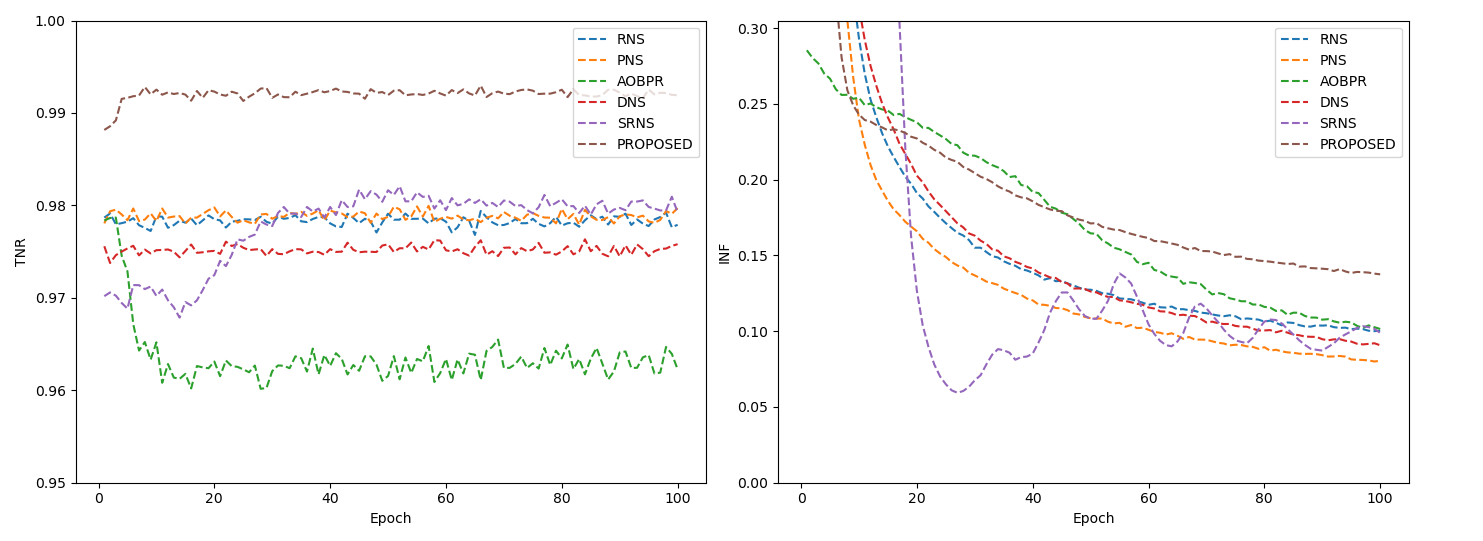
\includegraphics[width=\textwidth, height=0.35\textwidth]{3-tnr.png}
	\caption{不同方法的采样质量比较}
	\label{Fig:NegQua}
\end{figure*}
\subsubsection{负采样质量}
在本小结中,测试了两个采样准则:(i) 由公式\eqref{Eq:unbias}给出的\textit{后验概率准则}。(ii) 由公式\eqref{Eq:NegativeSam}给出的\textit{贝叶斯采样准则}。前者旨在选择真负样本,而后者旨在采样高质量的负样本实例。我们首先检查\textit{后验概率准则}是否能够选择真负样本实例,然后检查\textit{贝叶斯采样准则}是否能够选择高质量的负样本。

\textit{后验概率准则}通过从候选集$\mathcal{M}_u$中选择具有最大$\mathtt{unbias}(\cdot)$值的负样本实例来实现:
\begin{eqnarray} \label{Eq:PosteriorSam}
	j   &=&   \mathop{\arg\max}\limits_{l \in \mathcal{M}_u} \mathtt{unbias}(l)
\end{eqnarray}
$\mathcal{I}_u^-$是一个从$\mathcal{I}_u^-$中随机选择的负样本的小候选集,规模大小固定为5。\textit{贝叶斯采样准则}通过从候选集$\mathcal{M}_u$中选择具有最小条件采样风险$R(\cdot|i)$的负样本实例来实现:
\begin{eqnarray} \label{Eq:NegativeSam1}
	j  = \mathop{\arg\min}\limits_{l \in\mathcal{M}_u}~ \mathtt{info}(l)\cdot [1-(1+\lambda)\mathtt{unbias}(l)]
\end{eqnarray}
不同采样方法的采样质量展示在图~\ref{Fig:NegQua}中。

(i) 采样偏差:\textit{固定分布采样}(\textsf{RNS}和\textsf{PNS})表现相对中等。它们的真负样本率(TNR)在随机样本为真负样本的概率附近波动。\textit{困难负采样}(\textsf{AOBPR}和\textsf{DNS})表现最差。它们采用贪婪策略强调排名较高的负样本,也带来了更高的采样误差风险,正如我们在第~\ref{Sec:Dis}节中讨论的那样。\textsf{SRNS}利用预测分数方差的简单先验统计信息,限制了负样本分类的潜力,因为这种先验方差可能导致采样分布过于集中。提出的\textit{贝叶斯负采样}(\textsf{BNS})由于我们的贝叶斯负分类,TNR接近1,实现了最佳性能。

(ii) 采样质量:样本的信息量随训练时期的增加而降低。这是因为经过训练的推荐模型可能会将用户潜在感兴趣的伪负真负样本(参见图~\ref{Fig:DistributionStatistics})。在足够的训练时期后,\textsf{BNS}实现了最佳性能。\textit{困难负采样}(\textsf{AOBPR}和\textsf{DNS})受到最高采样偏差的惩罚更多。\textsf{SRNS}采用线性加权平均来结合信息性和方差,这可能不能保证采样无偏和信息丰富的实例

\subsubsection{超参数分析}\label{Appendix:Selection}
首先将候选集$\mathcal{M}_u$的大小固定为5,以研究$\lambda$对性能的影响。较大的$\lambda$值意味着更加强调来自真负样本的排名增益,而较小的$\lambda$值则更加关注避免采样假负样本的风险。从图~\ref{Fig:highperparameter}中可以观察到,当$\lambda$的值从0.1增加到1时,$NDCG@20$显著提高,并且在$\lambda=5$时达到最大值。

然后,将最优$\lambda$值固定为5,研究$\mathcal{M}_u$的大小对性能的影响,并在范围$\{1, 3, 5, 10, 15\}$内搜索$|\mathcal{M}_u|$的取值。需要注意的是,当$|\mathcal{M}_u|=1$时,提出的\textsf{BNS}变为经典的随机负采样(\textsf{RNS})。当$|\mathcal{M}_u|>1$时,贝叶斯采样准则开始发挥其样本筛选的作用。当$|\mathcal{M}_u|=|\mathcal{I}_u^-|$时,公式~\eqref{Eq:NegativeSam}中的采样器$h$是由公式~\eqref{Eq:OptimalSam}给出的最优采样器$h^*$。从图~\ref{Fig:highperparameter}中可以观察到,当$|\mathcal{M}_u|=5$或$10$时,$NDCG@20$达到最大值。为了降低时间复杂度,我们将$|\mathcal{M}_u|=5$。

\begin{figure*}[!]
	\centering
	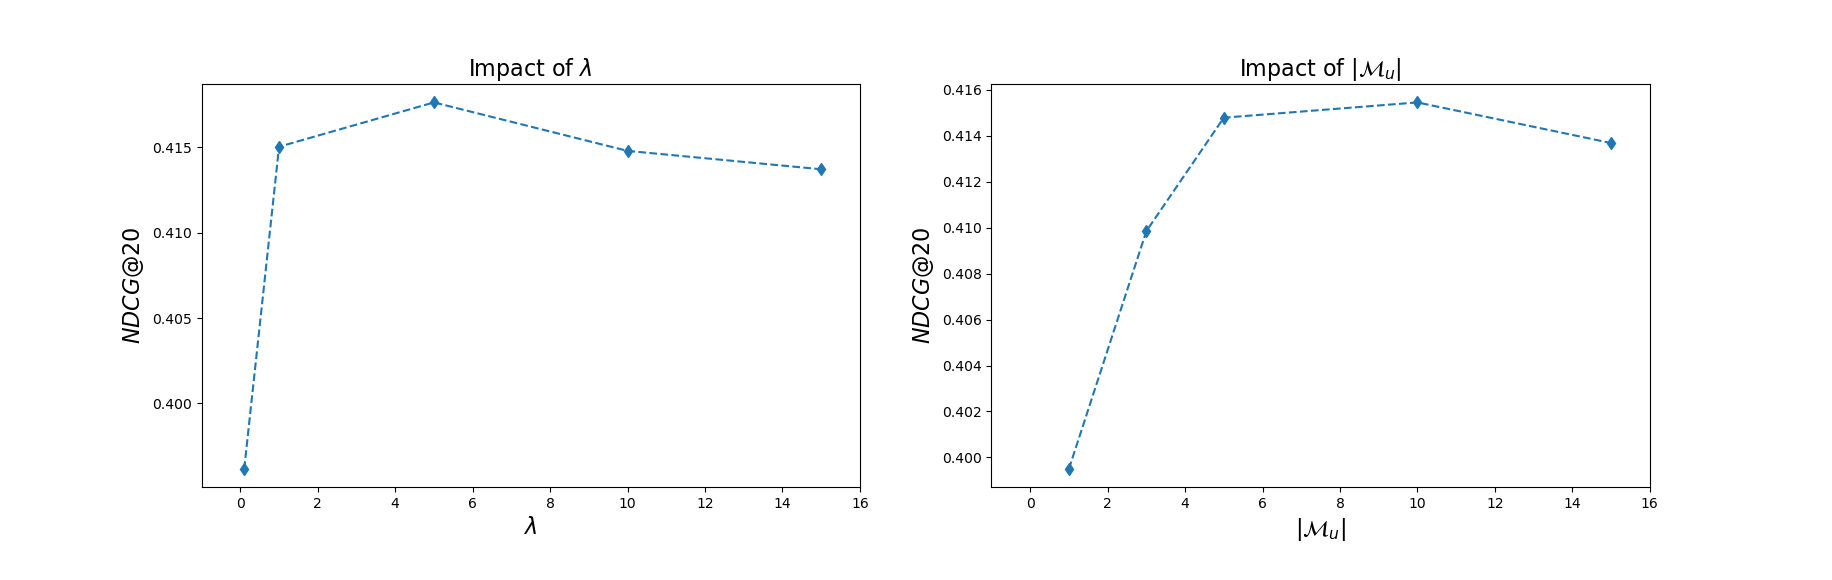
\includegraphics[width=\textwidth, height=0.3\textwidth]{3-highperparameter.png}
	\caption{参数$\lambda$和$|\mathcal{M}_u|$的影响}
	\label{Fig:highperparameter}
\end{figure*}
当$|\mathcal{M}_u| > 10$时,$NDCG@20$的值下降。这个实验结果与预期不符,因为$|\mathcal{M}_u|$值越大,越容易选择最优负样本。我们认为这是由于不可靠的先验概率$P_{fn}(l)$估计引起的。不可靠的先验信息进一步导致了由$F(\hat{x}_l)$表示的分类结果的偏差,进而导致了负信号$\mathtt{unbias}(\cdot)$的进一步偏离。过大的$|\mathcal{M}_u|$放大了负信号偏差的不利影响,导致性能下降。更多讨论可以在第~\ref{Appendix:Asymptotic}节中找到。

本节进一步研究了\textsf{BNS}对$\lambda$、样本信息$\hat{x}_l$和先验信息$P_{fn}(l)$的敏感性。
\begin{itemize}
	\item[-]\textsf{BNS}-1:$\lambda$的热启动。设置$\lambda = \max(10-\alpha \times \text{epoch}, 2)$,随着epoch数的增加,线性降低$\lambda$的值。即,在初始阶段,较大的$\lambda$强调对真负样本进行排名增益,而在后期阶段,较小的$\lambda$强调对假负样本进行采样损失。其中,$\alpha$选为0.1。
	\item[-]\textsf{BNS}-2:样本信息$\hat{x}_l$的热启动。我们首先采用\textsf{RNS}训练一个推荐模型一些epoch,以学习更可靠的样本信息$F(\hat{x}l)$,然后通过将其替换为我们的\textsf{BNS}来恢复训练。
	\item[-]\textsf{BNS}-3:无信息先验分布。对于这种情况,\textsf{BNS}简化为仅使用样本信息$\hat{x}l$进行负采样的\textsf{DNS}。对于单次随机试验,任何物品$l$被交互的概率为1/1682,即我们对任何负样本$l$无差别地设置$P_{fn}(l) = 1/1682$,其中1682是物品的总数。
	\item[-]\textsf{BNS}-4:职业信息增强的先验分布。在公式~\eqref{Eq:Prior}的基础上,我们添加了一个调整因子来改善$P_{fn}(l)$的估计:
	\[P{fn}(l) = \frac{pop_l}{N} \cdot (1 + \triangle o_{ul}),\]
	其中$\triangle o_{ul} = \frac{o_{ul} - \bar{o}l}{\max{o}{l}}$表示$u$的职业中对$l$的偏好次数与平均值之间的偏差。$o_{ul}$是具有与$u$相同职业的群体在物品$l$上的交互次数,$\bar{o}_l$是物品$l$被每个职业交互的平均次数。
\end{itemize}
实验结果见表~\ref{Exp:study}。以下是我们的发现:

\begin{table*}[h]
	\centering
	\caption{BNS负采样算法的消融实验}\label{Exp:study}
	\resizebox{1\textwidth}{!}{
		\begin{tabular}{lclccccccccccc}
			\toprule[1.2pt]
			\multirow{2}*{\textbf{Dataset}} & \multirow{2}*{\textbf{CF Model}} & \multirow{2}*{\textbf{ Method}} & \multicolumn{3}{c}{Top-5} &~& \multicolumn{3}{c}{Top-10}&~&\multicolumn{3}{c}{Top-20}\\ \cline{4-6} \cline{8-10} \cline{12-14}
			
			~ & ~ & ~ & Precision& Recall& NDCG& ~ &Precision& Recall& NDCG& ~ &Precision& Recall& NDCG \\ \hline
			
			\multirow{6}*{\textbf{100K}} & \multirow{6}*{\textbf{MF}} & RNS & 0.3900   &0.1301	&0.4143	&~&0.3363	&0.2164	&0.3967& ~&0.2724&0.3298&0.3962 \\
			~ & ~ & BNS    &0.4205	&0.1467	&0.4558&~	&0.3463	&0.2290	&0.4217& ~&0.2762&0.3466& 0.4176\\
			~ & ~ & BNS-1  &0.4237	&0.1471	&0.4551	&~&0.3495	&0.2305	&0.4238& ~&0.2762&0.3495&0.4197\\
			~ & ~ & BNS-2  &0.4148	&0.1456	&0.4449&~	&0.3411	&0.2245 &0.4132& ~&0.2738&0.3434&0.4125\\
			~ & ~ & BNS-3  &0.4048	&0.1392	&0.4266&~	&0.3423	&0.2282 &0.4043& ~&0.2720&0.3406&0.4030\\
			~ & ~ & BNS-4  &0.4262	&0.1478	&0.4566&~	&0.3486	&0.2305 &0.4235& ~&0.2792&0.3520&0.4216\\
			\cline{1-14}
			
			\bottomrule[1.2pt]
			
		\end{tabular}
	}
\end{table*}

%########################
\textbf{\textsf{BNS}对$\lambda$的敏感性}:$\lambda$的热启动取得了更好的性能(\textsf{BNS}-1)。较大的$\lambda$值意味着在采样风险和增益之间的权衡程度更高,即更加强调来自真负样本的排名增益而非假负样本的风险。结果显示,对于模型学习来说,困难样本是重要的,这与现有研究的发现一致~\cite{Ding:2020:NIPS,Park:2019:WWW}。建议采用$\lambda$的热启动策略:在初始阶段使用较大的值强化对困难样本的采样,而在后期阶段使用较小的$\lambda$以避免采样伪负例。

\textbf{\textsf{BNS}对先验概率$P_{fn}(\cdot)$的敏感性}:结果显示,在没有先验信息的情况下,\textsf{BNS-3}相对于标准的\textsf{BNS}性能较差,而在增强职业信息先验概率的情况下,\textsf{BNS-4}相对于标准的\textsf{BNS}性能更好。结果表明,\textsf{BNS}对先验概率敏感。先验信息影响负采样的机制是:不可靠的先验概率$P_{fn}(\cdot)$导致由$F(\hat{x}_\cdot)$表示的分类结果偏差,进而导致负信号$\mathtt{unbias}(\cdot)$的进一步偏离。过大的候选集$\mathcal{M}u$放大了负信号偏差的不利影响,导致性能下降。因此,如果先验概率$P{fn}(\cdot)$可靠,则选择更大的$\mathcal{M}_u$更好;否则,应选择适度大小的$\mathcal{M}u$。特别地,在非信息先验分布的情况下,\textsf{BNS}等效于\textsf{DNS}:\textsf{BNS}采样具有适当$F(\hat{x})$值的实例,而\textsf{DNS}采样具有适当排名位置的实例,而$F(\hat{x})$和排名位置具有一对一的映射关系。通过选择适当的$|\mathcal{M}u|$和$\lambda$,\textsf{BNS-3}的性能与\textsf{DNS}相当。我们建议选择最可靠的先验信息来建模$P{tn}(\cdot)$或$P{fn}(\cdot)$。

\textbf{\textsf{BNS}对样本信息$\hat{x}_l$的敏感性}:样本信息$\hat{x}$的热启动(\textsf{BNS-2})并没有像预期的那样取得更好的性能,我们认为有三个原因:(i) 初始训练阶段的随机采样难以采样到难负例,导致\textsf{BNS-2}的性能下降;(ii) $\hat{x}$是由先验概率和采样器$h$内生确定的,因此$\hat{x}$的热启动对最终的排名性能影响有限;(iii) 我们使用样本信息$F(\hat{x}\cdot)$的方式对$\hat{x}_\cdot$的微小变化不敏感,因此改进的$\hat{x}$对提高采样质量的影响有限。我们认为\textsf{BNS}具有对不同排名模型的鲁棒性,这是它对不同排名模型具有鲁棒性的重要体现,因为在不满足顺序关系的条件下(例如早期训练阶段或弱排名模型),\textsf{BNS}仍然能够利用先验信息采样高质量的负实例。

\subsubsection{向其他损失函数推广}\label{Appendix:LossFunc}
本小结检验\textsf{BNS}在其他损失函数中的适用性。我们选择了两个基于对比的损失函数,即二元交叉熵(BCE)损失和InfoNCE损失函数。我们使用矩阵分解模型作为编码器,并分别将BPR损失~\cite{Steffen:2009:UAI}替换为BCE损失~\cite{Zizhuo:2021:ICDM}和Info-NCE~\cite{Oord:2018:arxiv}损失。超参数保持与使用BPR损失时相同。具体而言,InfoNCE损失的负实例数量$N$固定为2。表~\ref{Exp:supp}展示了使用不同损失函数的结果。可以看出,与随机负采样\textsf{RNS}相比,\textsf{BNS}在所有三个损失函数中都取得了显著的改进,展示了\textsf{BNS}的良好适用性。
\begin{table*}[h]
	\centering
	\caption{不同损失函数下BNS负采样算法的表现}\label{Exp:supp}
	\resizebox{1\textwidth}{!}{
		\begin{tabular}{lclcccccccccccc}
			\toprule[1.2pt]
			
			\multirow{2}*{\textbf{Dataset}} & \multirow{2}*{\textbf{CF Model}} & \multirow{2}*{\textbf{Loss Function}} \multirow{2}*{\textbf{Method}} & \multicolumn{3}{c}{Top-5} &~& \multicolumn{3}{c}{Top-10}&~&\multicolumn{3}{c}{Top-20}\\ \cline{5-7} \cline{9-11} \cline{13-15}
			
			~ & ~ & ~ &~& Precision& Recall& NDCG& ~ &Precision& Recall& NDCG& ~ &Precision& Recall& NDCG \\ \hline
			
			\multirow{6}*{\textbf{100K}} & \multirow{6}*{\textbf{MF}} & \multirow{2}*{\textbf{BPR}} &RNS & 0.3900   &0.1301	&0.4143	&~&0.3363	&0.2164	&0.3967& ~&0.2724&0.3298&0.3962 \\
			
			~ & ~ & ~&BNS    &0.4205	&0.1467	&0.4558&~	&0.3463	&0.2290	&0.4217& ~&0.2762&0.3466& 0.4176\\\cline{3-15}
			
			~ & ~ & \multirow{2}*{\textbf{BCE}}&RNS    &0.3917	&0.1329	&0.4107&~	&0.3339	&0.2187	&0.3923& ~&0.2696&0.3315&0.3928\\
			~ & ~ & ~&BNS    &0.4226	&0.1454	& 0.4490&~	&0.3514&0.2299	&0.4205& ~&0.2821&0.3482& 0.4182\\\cline{3-15}
			~ & ~ & \multirow{2}*{\textbf{Info NCE}}&RNS    &0.3923	&0.1322	&0.4193&~	&0.3353	&0.2162	&0.3988& ~&0.2728&0.3376& 0.4012\\
			~ & ~ & ~&BNS    &0.4241	& 0.1471	&0.4523&~	&0.3519	&0.2281	&0.4226& ~&0.2817&0.3467& 0.4195\\
			\cline{1-15}
			
			\bottomrule[1.2pt]
			
		\end{tabular}
	}
\end{table*}

\subsubsection{渐近最优采样器}\label{Appendix:Asymptotic}
本小结展示所提出的采样器$h$通过理想先验概率$P_{fn}(l)$以渐进最优采样器$h^*$的过程。设置$P_{fn}(l) = (label(l)-0.2)^2$,即如果$l\in fn$,则$P_{fn}(l)=0.64$,否则$P_{fn}(l)=0.04$。通过逐渐增加$\mathcal{M}_u$的大小,以渐近最优采样器,其中$\lambda$固定为5。模拟结果如表~\ref{Table:asymptoticprocess}所示。通过增加候选集的大小,可以实现最优采样器$h^*$而不会降低排名性能。该结果验证了我们在第~\ref{Appendix:Selection}节中的分析。在具备一定程度的先验信息的情况下,即使对于简单的基于点乘的表示学习方法,\textsf{BNS}也能取得可观的性能,展示了负采样研究的巨大潜力。最优采样器(即$|\mathcal{M}_u| = |\mathcal{I}_u^-|$)的性能是基于点乘模型的经验上界。由于存在低秩约束和矩阵分解的有限表达能力,推荐性能无法达到1。
\begin{table*}[h]
	\centering
	\caption{向最优采样器的渐进过程}\label{Table:asymptoticprocess}
	\resizebox{1\textwidth}{!}{
		\begin{tabular}{lclccccccccccc}
			\toprule[1.2pt]
			\multirow{2}*{\textbf{Dataset}} & \multirow{2}*{\textbf{CF Model}} & \multirow{2}*{\textbf{\textsf{BNS} Size}} & \multicolumn{3}{c}{Top-5} &~& \multicolumn{3}{c}{Top-10}&~&\multicolumn{3}{c}{Top-20}\\ \cline{4-6} \cline{8-10} \cline{12-14}
			
			~ & ~ & ~ & Precision& Recall& NDCG& ~ &Precision& Recall& NDCG& ~ &Precision& Recall& NDCG \\ \hline
			
			\multirow{9}*{\textbf{100K}} & \multirow{9}*{\textbf{MF}} & $|\mathcal{M}_u| = 1$ & 0.3900   &0.1301	&0.4143	&~&0.3363	&0.2164	&0.3967& ~&0.2724&0.3298&0.3962 \\
			~ & ~ & $|\mathcal{M}_u| = 3$  &0.4909	&0.1567&0.5211&~	&0.4220	&0.2565	&0.4942& ~&0.3366&0.3872&0.4856\\
			~ & ~ & $|\mathcal{M}_u| = 5$ &0.5109	&0.1612	&0.5422	&~&0.4329	&0.2602	&0.5092& ~&0.3456&0.3925&0.4992\\
			~ & ~ & $|\mathcal{M}_u| = 10$  &0.5351	&0.1696	&0.5685&~	&0.4589	&0.2722 &0.5365& ~&0.3663&0.4081&0.5245\\
			~ & ~ & $|\mathcal{M}_u| = 20$  &0.5760	&0.1828	&0.6070&~	&0.4885	&0.2875 &0.5695& ~&0.3830&0.4196&0.5498\\
			~ & ~ & $|\mathcal{M}_u| = 50$  &0.6239	&0.1989	&0.6599&~	&0.5252	&0.3049 &0.6146& ~&0.4031&0.4312&0.5843\\
			~ & ~ & $|\mathcal{M}_u| = 100$   &0.6509	&0.2104	&0.6898&~	&0.5382	&0.3125 &0.6346& ~&0.4053&0.4321&0.5971\\
			~ & ~ & $|\mathcal{M}_u|= 500$  &0.6661	&0.2183	&0.7128&~	&0.5412	&0.3131 &0.6487& ~&0.4041&0.4300& 0.6076\\
			~ & ~ & $|\mathcal{M}_u|= |\mathcal{I}_u^-|$  &0.6674	&0.2184	&0.7133&~	&0.5429	&0.3140 &0.6495& ~&0.4041& 0.4292&0.6073\\
			\cline{1-14}
			
			\bottomrule[1.2pt]
			
		\end{tabular}
	}
\end{table*}

这些基准结果包括两个有启发性的消融实验的结果:(i) 只使用先验信息(物品流行度)的\textsf{PNS},以及 (ii) 只使用样本信息 $\hat{x}l$ 的\textsf{DNS}、\textsf{AOBPR}和\textsf{SRNS}。特别地,在无信息的先验分布的情况下,\textsf{BNS}退化为\textsf{DNS}。\textsf{BNS}根据适当的 $F(\hat{x})$-值对实例进行采样,而\textsf{DNS}根据适当的排名位置对实例进行采样,由于 $F(\hat{x})$ 和排名位置具有一对一的映射关系,因此它们实现了可比较的性能。上述两种范式的缺点是显而易见的:前者可以融合领域知识,但独立于模型状态,导致了静态的采样分布;后者利用了样本信息,但忽略了先验知识,在富有辅助信息的场景中,这将导致性能下降。所提出的\textsf{BNS}从贝叶斯的角度结合了先验信息和样本信息,并以赋予负信号$\mathtt{unbias}(l)$以后验概率的内涵。本章认为\textsf{BNS}的性能改进源于三个方面:(i) 先验信息 $P{tn}(l)$ 或 $P_{fn}(l)$,以及 (ii) 使用样本信息 $\hat{x}_l$。(iii) \textsf{BNS}是最小化经验采样风险的理论最优采样器。

\section{本章小结}\label{Sec:Conclusion}
本章定义了一个与模型无关的后验概率估计,作为定量的负信号度量。而后提出了贝叶斯负采样规则,这是最小化经验采样风险的理论最优的采样规则。\textsf{BNS}的贡献在于以后验概率的意义上指定了负信号度量。从贝叶斯的角度,\textsf{BNS}通过结合静态的先验信息和动态的样本信息,统一了现有的两种提取负信号的范式。需要注意的是,\textsf{BNS}并未具体指定建模先验概率的方法。相反,$P_{tn}(l)$(或$P_{fn}(l)$)为使用辅助信息建模先验概率的方法提供了接口。此外,只要模型旨在将正例的得分高于负例,\textsf{BNS}也可以应用于其他基于对比的损失函数。

需要指出的是,负采样算法与基于GPU批量并行计算Mini-Batch模型并不兼容。典型的动态负采样需要先计算当前轮次样本得分(正向传播),然后采样负例。而基于Mini-Batch模型需要把样本固定到DataLoader中,才能进行正向传播预测得分,这与动态负采样机制有所冲突。而动态负采样需要先得到预测得分,然后再采样负例。通常是把很多的候选负样本装载入Dataloader,并计算额外样本的预测得分来实现动态负采样,造成了额外的计算和存储开销。此外,本章所假设的真负例和伪负例的相似度分数的序关系是一个理想的情况,是一个比较强的假设。后面的章节将解决这两个局限性。
